\documentclass[11pt, a4paper]{article}
\usepackage{tikz}
\usetikzlibrary{positioning}
%----------Title Page---------
\title{
    The Role of Gradients in Convolutional Neural Networks\\~\\
    \large LeNet and the Use of Gradient Descent in Machine Learning}
\author{
    Maxwell Banks
}
\date{May 9, 2024}
%-----------------------------

\begin{document}
\maketitle
\newpage
\section{Background: Neural Networks}
Neural networks are a machine learning architecture commonly used for pattern recognition. Named for their 
similarity to human brains, traditional neural networks break inputs are composed of groups of nodes (called 
\textit{layers} of \textit{neurons}). Each node in a layer is connected to nodes in the preceding and following
layers, and contains some innate value (called a \textit{weight}). To process data with a neural network, data
is broken into discrete chunks that are fed into the first (input) layer of neurons. These neurons mutate the 
input according to their weight, then pass the result to the next (hidden) layer to continue the process. This 
process continues until the final (output) layer, wherein each node outputs a single number. These numbers can 
be used to classify inputs--for example, a neural net classifying images into "dog" or "cat" might have two
output nodes $O_1$ and $O_2$ corresponding to "dog" and "cat" respectively. The classification of an image into
"dog" or "cat" would be decided by $max(O_1, O_2)$. \\
\begin{center}
    \textbf{A Simple Diagram of a Neural Network}\\
    

\tikzset{%
  every neuron/.style={
    circle,
    draw,
    minimum size=1cm
  },
  neuron missing/.style={
    draw=none, 
    scale=4,
    text height=0.333cm,
    execute at begin node=\color{black}$\vdots$
  },
}

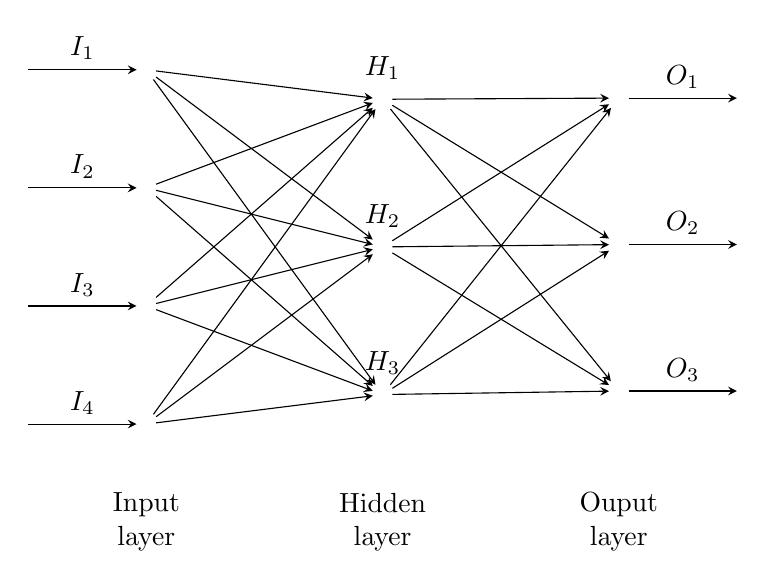
\begin{tikzpicture}[x=1.5cm, y=1.5cm, >=stealth]

\foreach \m/\l [count=\y] in {1,2,3,4}
  \node [every neuron/.try, neuron \m/.try] (input-\m) at (0,2.5-\y) {};

\foreach \m [count=\y] in {1,2,3}
  \node [every neuron/.try, neuron \m/.try ] (hidden-\m) at (2,2.5-\y*1.25) {};

\foreach \m [count=\y] in {1,2,3}
  \node [every neuron/.try, neuron \m/.try ] (output-\m) at (4,2.5-\y*1.24) {};

\foreach \l [count=\i] in {1,2,3,4}
  \draw [<-] (input-\i) -- ++(-1,0)
    node [above, midway] {$I_\l$};

\foreach \l [count=\i] in {1,2,3}
  \node [above] at (hidden-\i.north) {$H_\l$};

\foreach \l [count=\i] in {1,2,3}
  \draw [->] (output-\i) -- ++(1,0)
    node [above, midway] {$O_\l$};

\foreach \i in {1,...,4}
  \foreach \j in {1,...,3}
    \draw [->] (input-\i) -- (hidden-\j);

\foreach \i in {1,...,3}
  \foreach \j in {1,...,3}
    \draw [->] (hidden-\i) -- (output-\j);

\foreach \l [count=\x from 0] in {Input, Hidden, Ouput}
  \node [align=center, below] at (\x*2,-2) {\l \\ layer};

\end{tikzpicture}


\end{center}

\section{Historical Event}
This historical event analyzed by this paper is the publication of \textit{Gradient-Based Learning Applied to Document Recognition} (LeCun et al., 1998).
This paper revolutionized the training of neural networks and is the antecedent to much of the modern field of 
machine learning. 

\section{Summary}
The breakout research paper \textit{Gradient-Based Learning Applied to Document Recognition} (LeCun et al., 1998)
outlined LeNet-5, one of the first published instances of a Convolutional Neural Network (CNN). CNNs are a subtype
of neural network that generally specialize in image recognition (this is not univerally true, but for brevity this
paper will assume inputs are pixels of an image). LeCun et al. (1998) discusses using gradient-based learning 
techniques to train neural networks in recognizing letters, highlighting a variety of network architectures 
and explaining the effectiveness of gradient-based learning in the context of those architectures. \\

LeCun et al. (1998) had wide-ranging impacts on the field of machine learning as a whole, but perhaps the most 
notable impact was the popularization of CNNs trained using gradient-based learning. As the paper itself notes, 
"Gradient-Based Learning procedures have been used since the late 1950's, but they were mostly limited to 
linear systems." (LeCun et al. 1998)  The key innovation of LeCun et at. (1998) was to apply gradient-based 
learning (specifically, gradient descent) as a training mechanism for CNNs by using gradient descent to determine
the adjustment of node weights by minimizing the "loss function", a function representing how incorrect a neural 
network's guess was.\\

Gradient descent is a technique that dates back to Augustin-Louis Cauchy who outlined the technique in his pamphlet 
\textit{M\'ethode g\'en\'erale pour la r\'esolution des syst\`emes d'\'equations simultan\'ees} (Cauchy, 1847/2010). Cauchy described this technique as "...a general 
method which may be able to serve to resolve directly a system of simultaneous equations", and was mostly concerned
with using it to determine the movement of a star with precision. This technique minimizes a system of equations by repeatedly
calculating the gradient (interestingly, the paper itself does not appear to use the term gradient--it exclusively
uses partial derivatives) at a point, then "stepping" in the opposite direction of the gradient to a "lower" point. This 
process is repeated until a minimum is reached. 



\section{Explanation of Enhancement}
Explain in detail how the concepts utilized have directly led to innovations in our world that have made lives better for certain individuals, communities, nations, or the entire world

\section{Calculus Steps}
Explain the calculations utilized showing either a portion or all of the steps within the calculations.

\section{What If...}


\section{Bibliography}
http://vision.stanford.edu/cs598_spring07/papers/Lecun98.pdf
https://cs.uwaterloo.ca/~y328yu/classics/cauchy-en.pdf


\end{document}